%!TEX root=../../main.tex


\subsection{PageRank}
\subsubsection{Single-Node}

Ligra and Polymer support both regular and Delta-PageRank variants.
Ligra's regular PR implementation is faster on 4 of 7 graphs. If the regular version is slower than delta, that is only by a small difference. Explicitly, regular is slower than delta by 19\%\ on twitter, 17\%\ on rMat27 or 6\%\ for friendster. For the other graphs, the delta version is slower by a far greater margin, 50\%\ on flickr, 45\%\ on orkut, 13\%\ on wikipedia and 68\% on rMat28.
Hence, we only show the results of Ligra's regular PageRank implementation in our evaluation.
For Polymer we found the delta version to be faster on all graphs except rMat28. Delta-PR is on average 15\%\ faster on the first six graphs, while only being 0.3\%\ slower on rMat28.
Thus, the following only shows Polymer's faster Delta-PR implementation.


\todo{Hier fehlt noch Giraph, daher noch keine vollständige Auswertung.}

\begin{figure*}
	\begin{subfigure}{0.3\textwidth}
		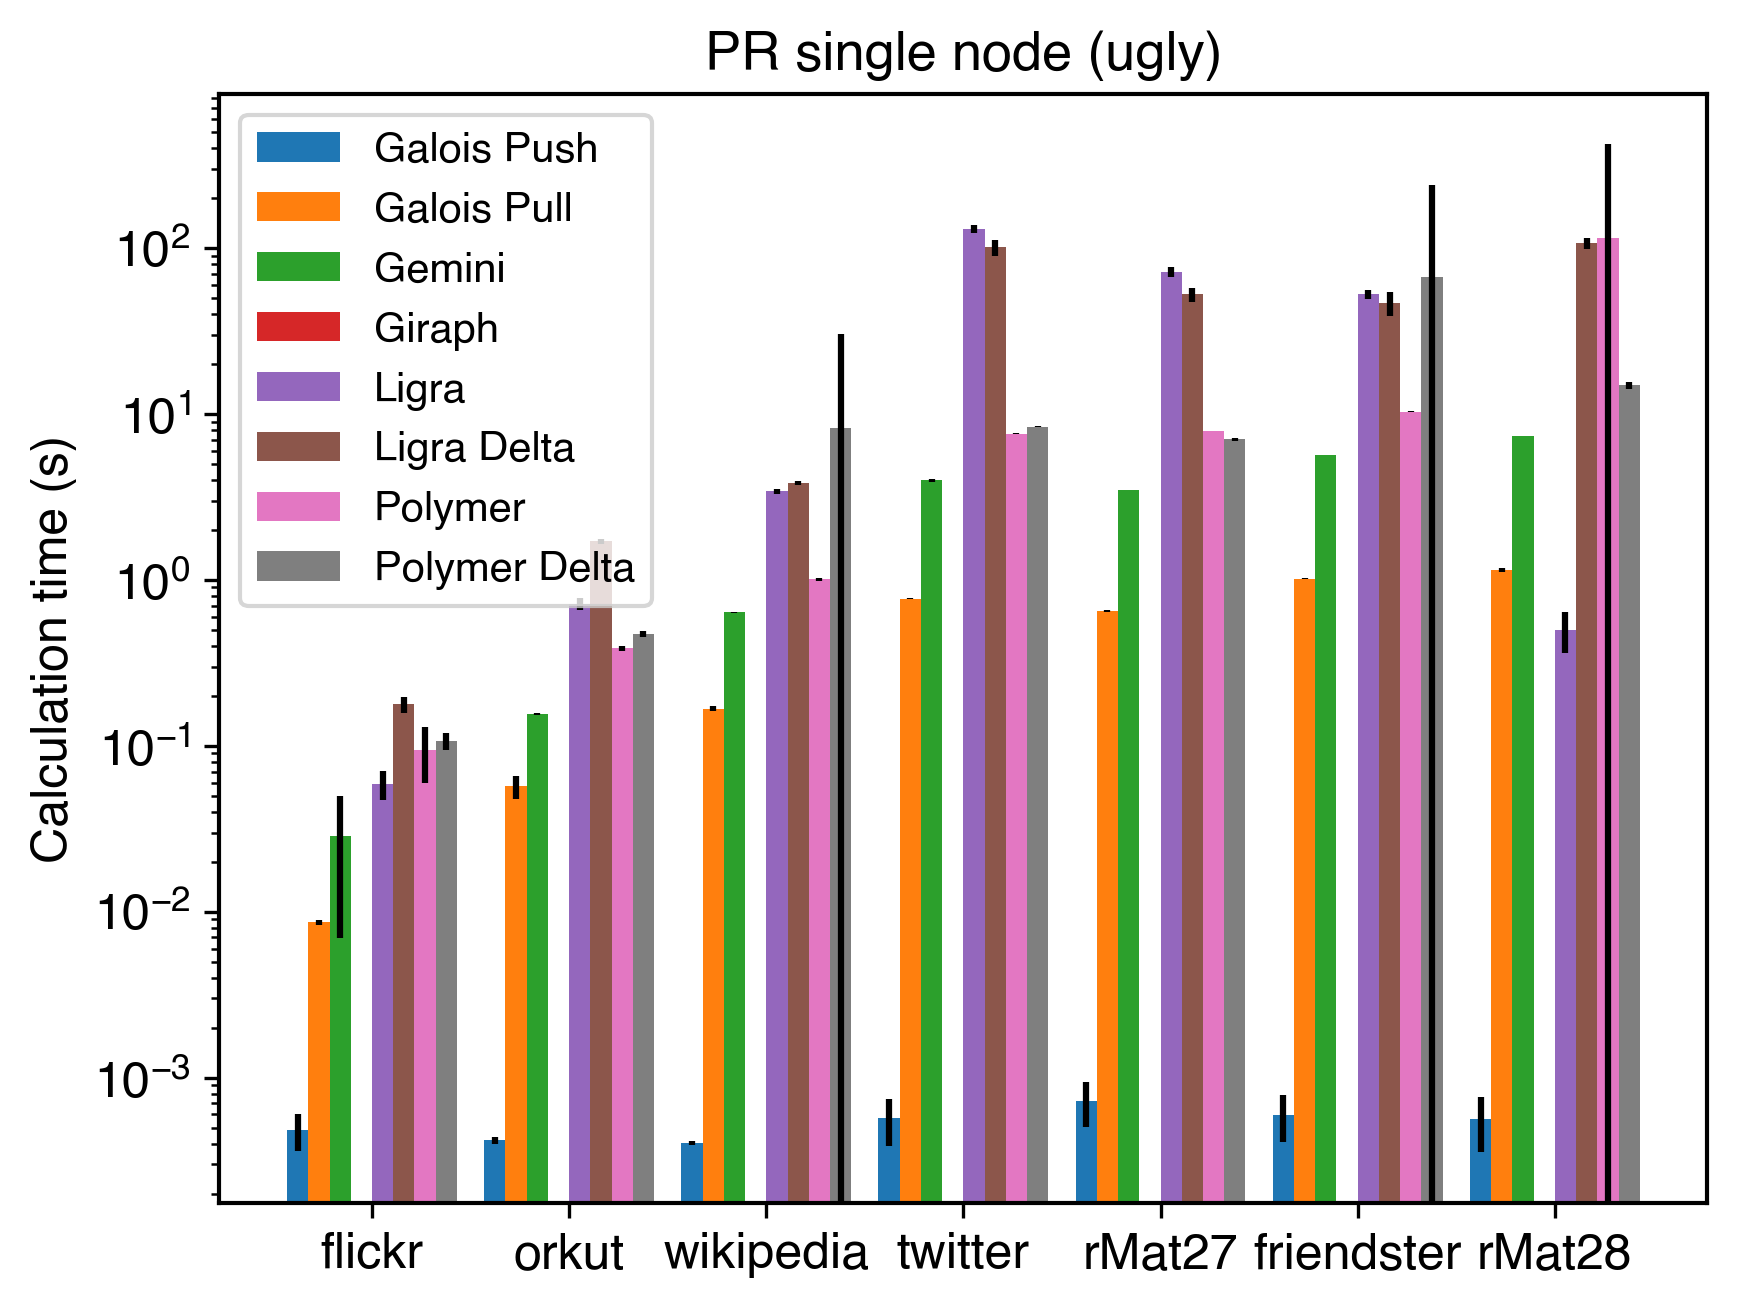
\includegraphics[width=\linewidth]{../../plots/singleNodePR_calcTime.png}
		\caption{Calculation times for PR on a single node}
		\label{fig:singleNodePR_calc}
	\end{subfigure}
	\hfil
	\begin{subfigure}{0.3\textwidth}
		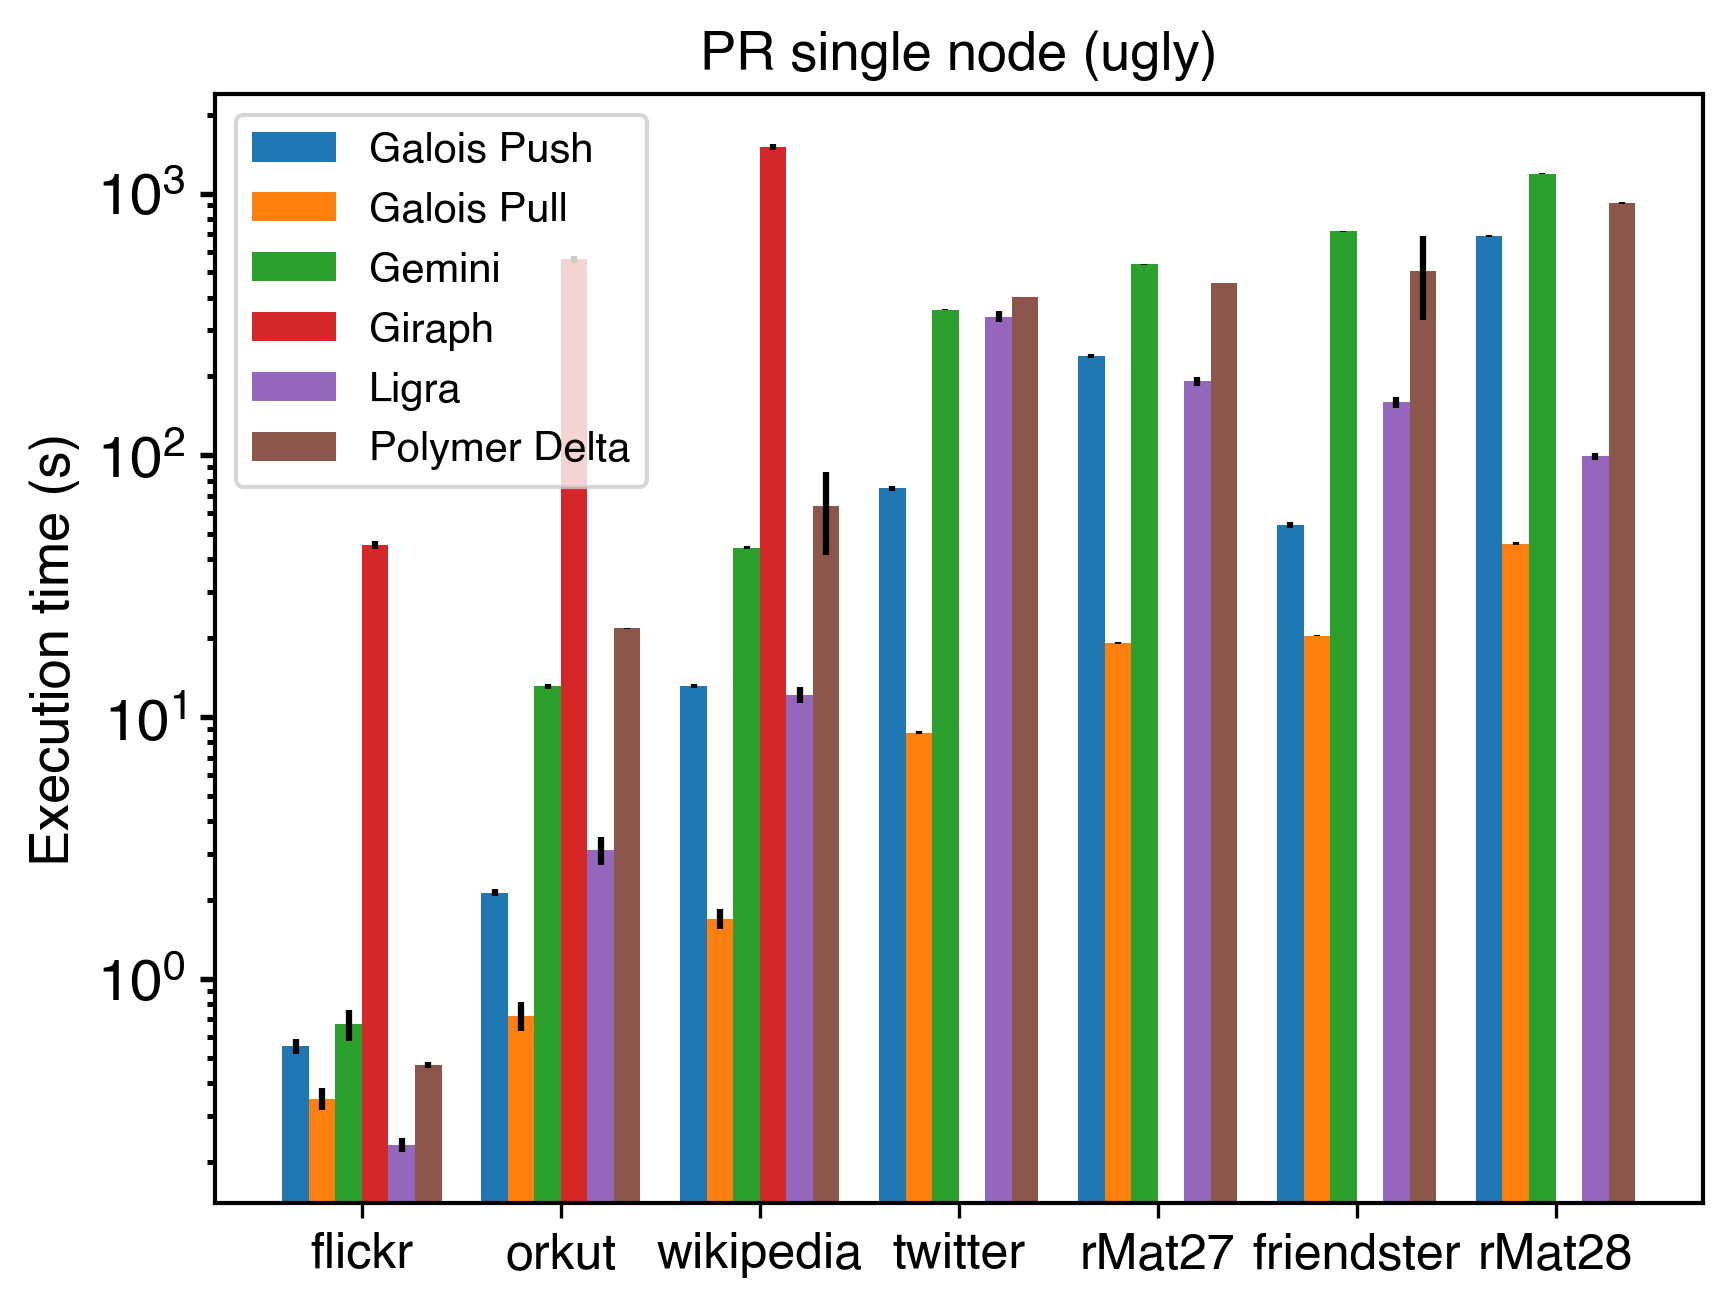
\includegraphics[width=\linewidth]{../../plots/singleNodePR_execTime.png}
		\caption{Execution times for PR on a single node}
		\label{fig:singleNodePR_exec}
	\end{subfigure}
	\hfil
	\begin{subfigure}{0.3\textwidth}
		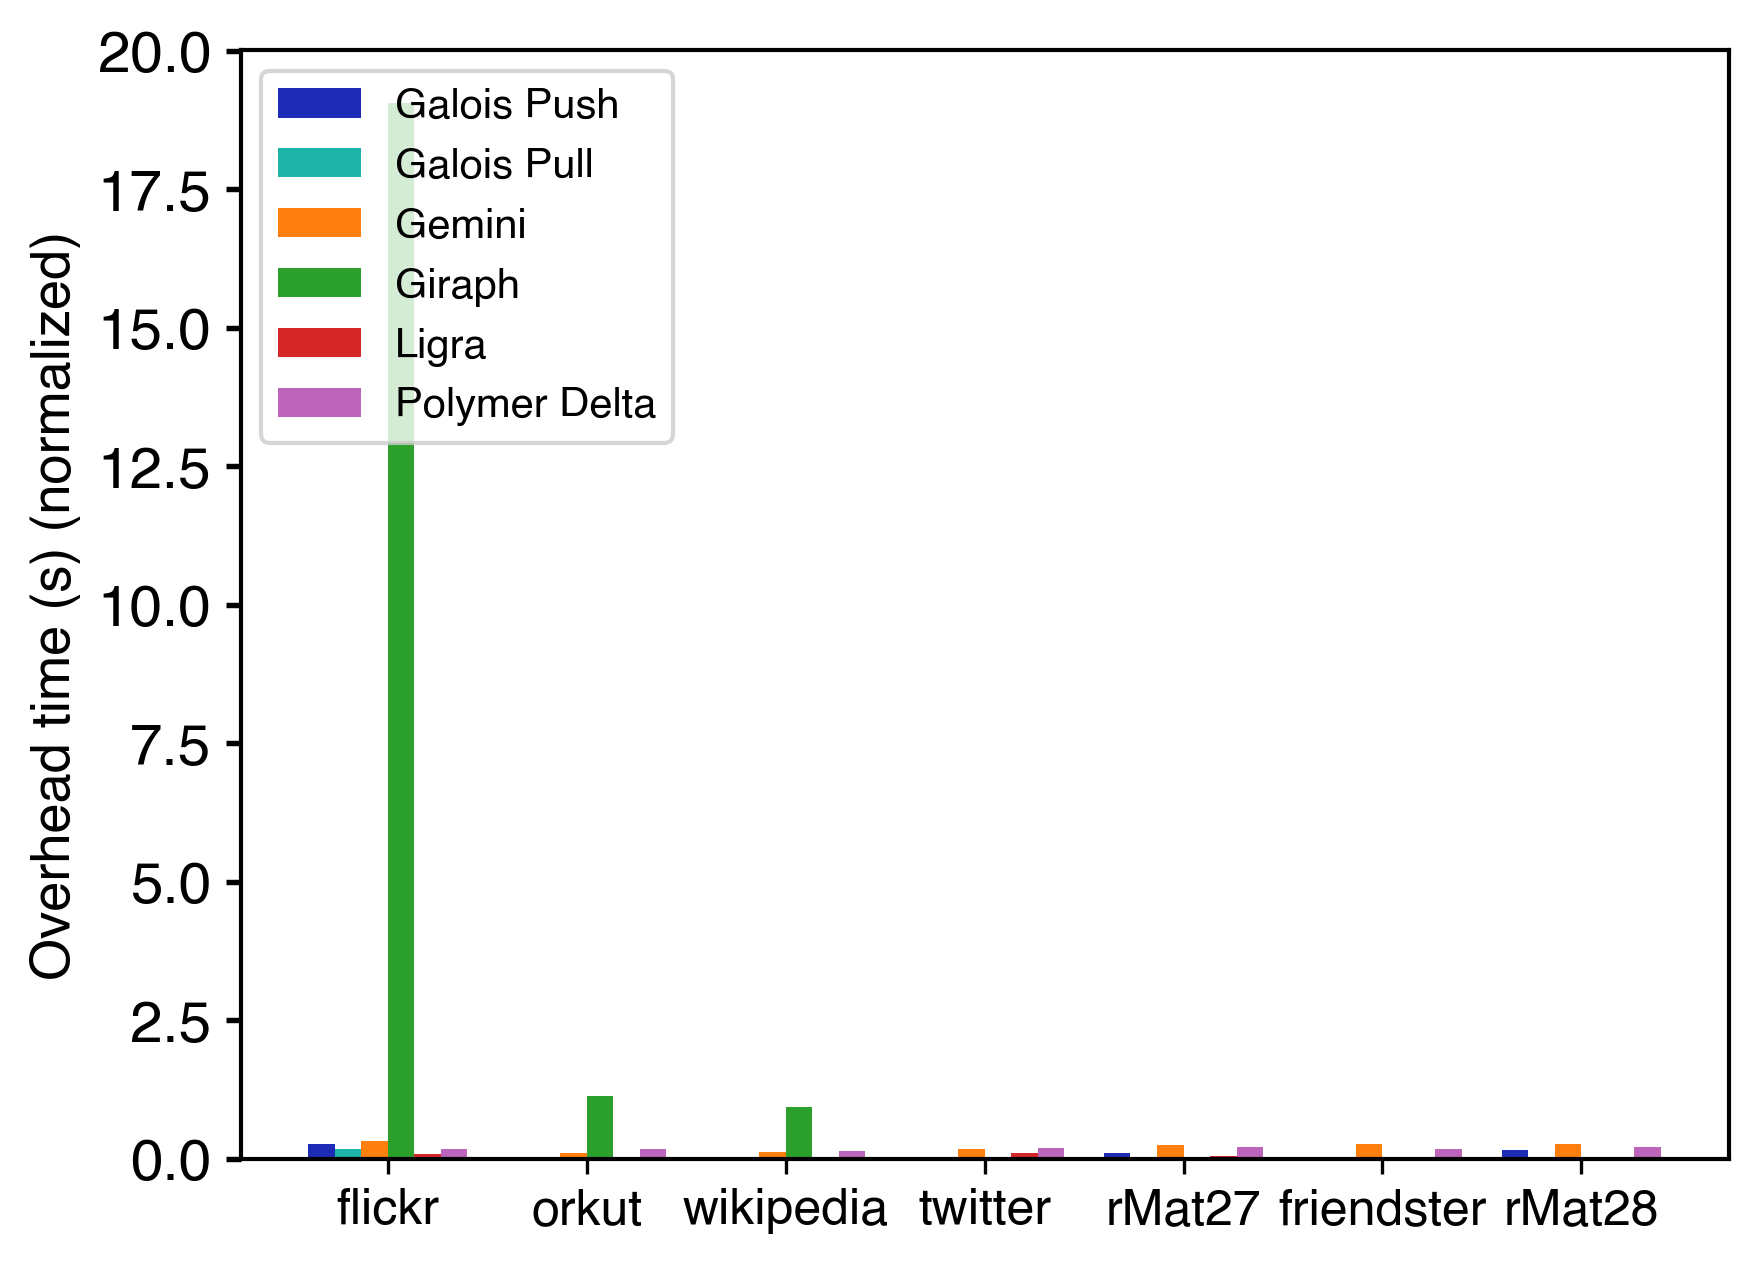
\includegraphics[width=\linewidth]{../../plots/singleNodePR_overheadTimeNormalized.png}
		\caption{Overhead time normalized by the graph size in million edges}
		\label{fig:singleNodePR_overheadNormalized}
	\end{subfigure}

	\caption{Average times on a single computation node, black bars represent one standard deviation in our testing}
\end{figure*}



\subsubsection{Distributed}
The \autoref{fig:distributedPR} shows our results of PageRank on the distributed cluster.
First of all, Giraph was unable to complete the test because it required more than 250GB of RAM for rMat28. Thus this results is missing.
When comparing the calculation times in \autoref{fig:distributedPR_calc} to the execution times in \autoref{fig:distributedPR_exec}, we see similar behaviour of all frameworks. This means that unlike with SSSP or BFS, the calculation times and execution times are similar with respect to the relations of the frameworks to one another. More specifically, there are no overhead outliers like it was the case with Giraph on SSSP.

\begin{figure*}
	\begin{subfigure}{0.3\textwidth}
		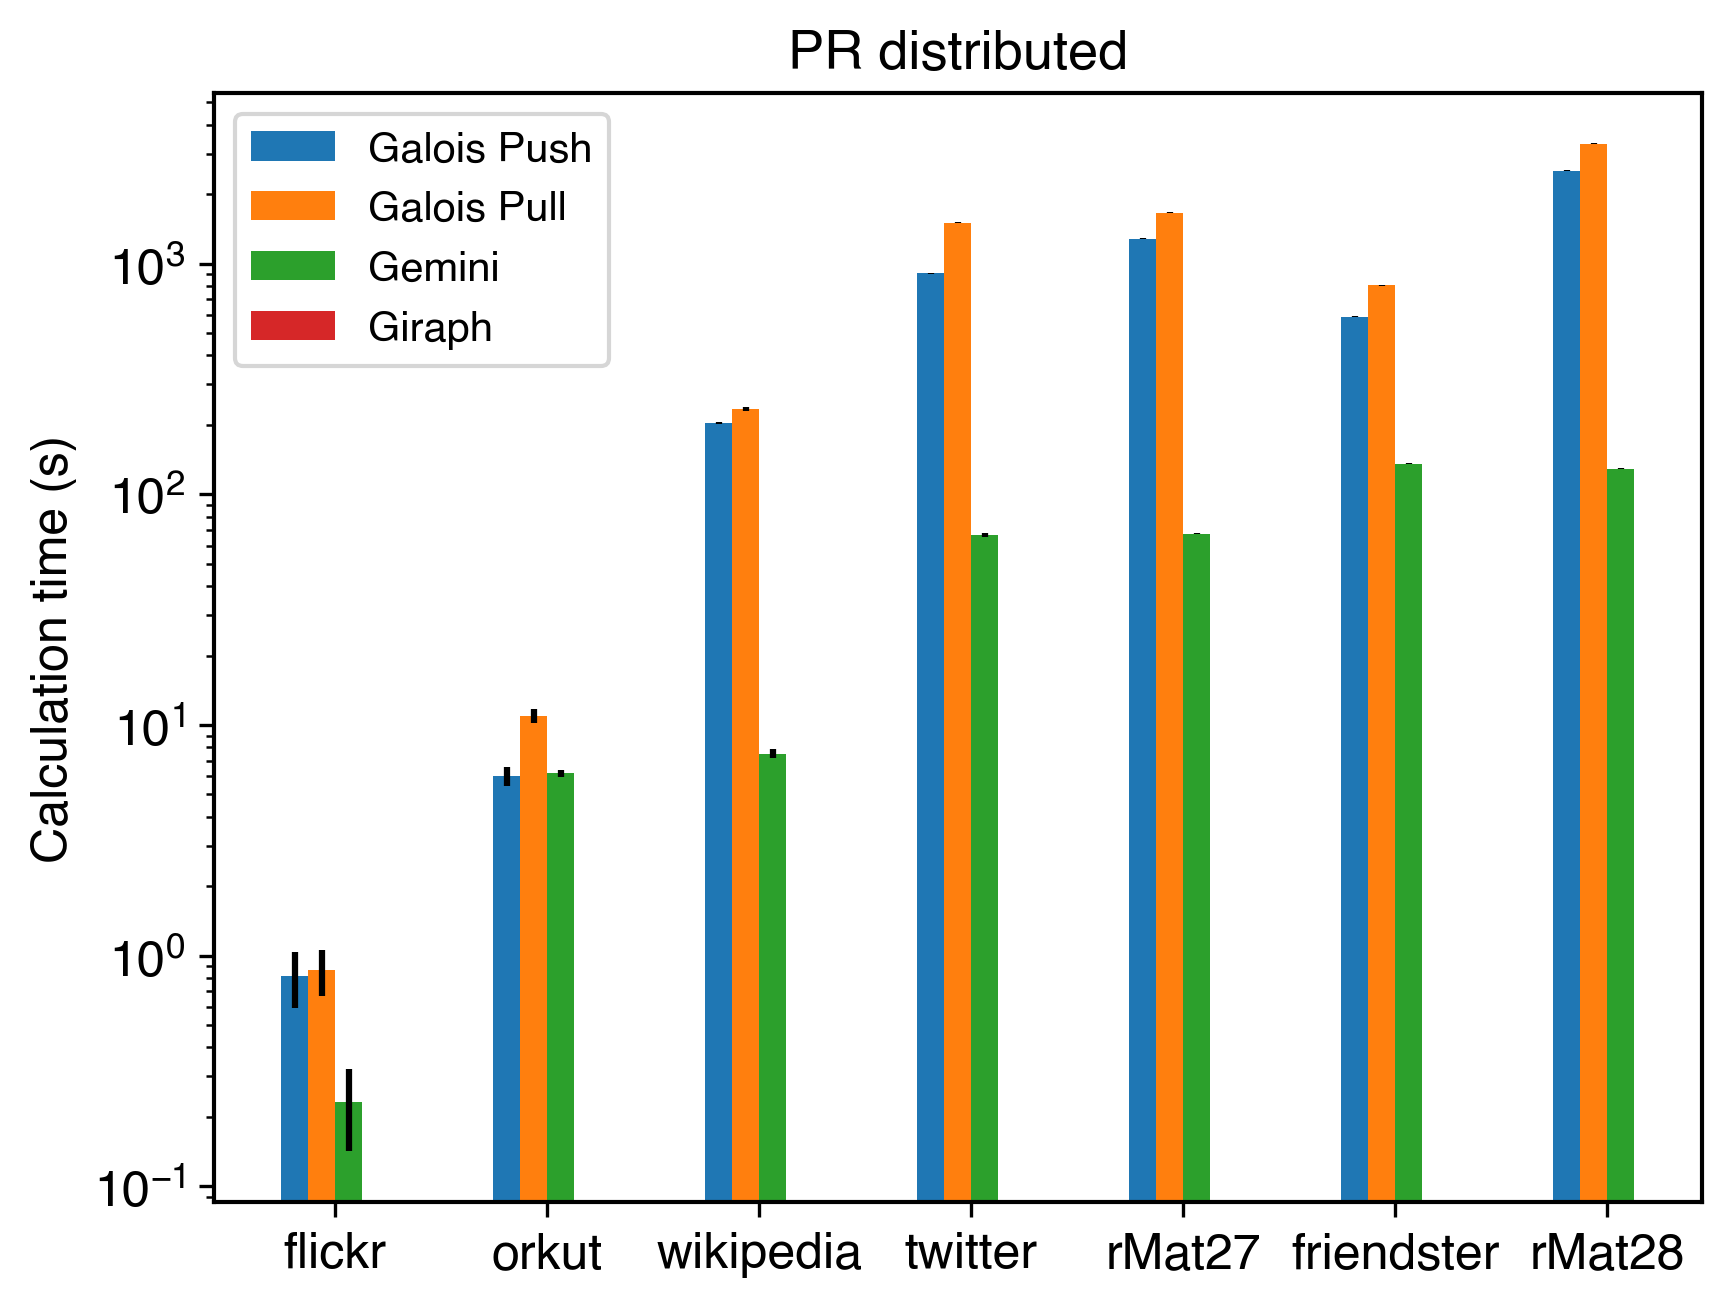
\includegraphics[width=\linewidth]{../../plots/distributedPR_calcTime.png}
		\caption{Calculation times for distributed PR}
		\label{fig:distributedPR_calc}
	\end{subfigure}
	\hfil
	\begin{subfigure}{0.3\textwidth}
		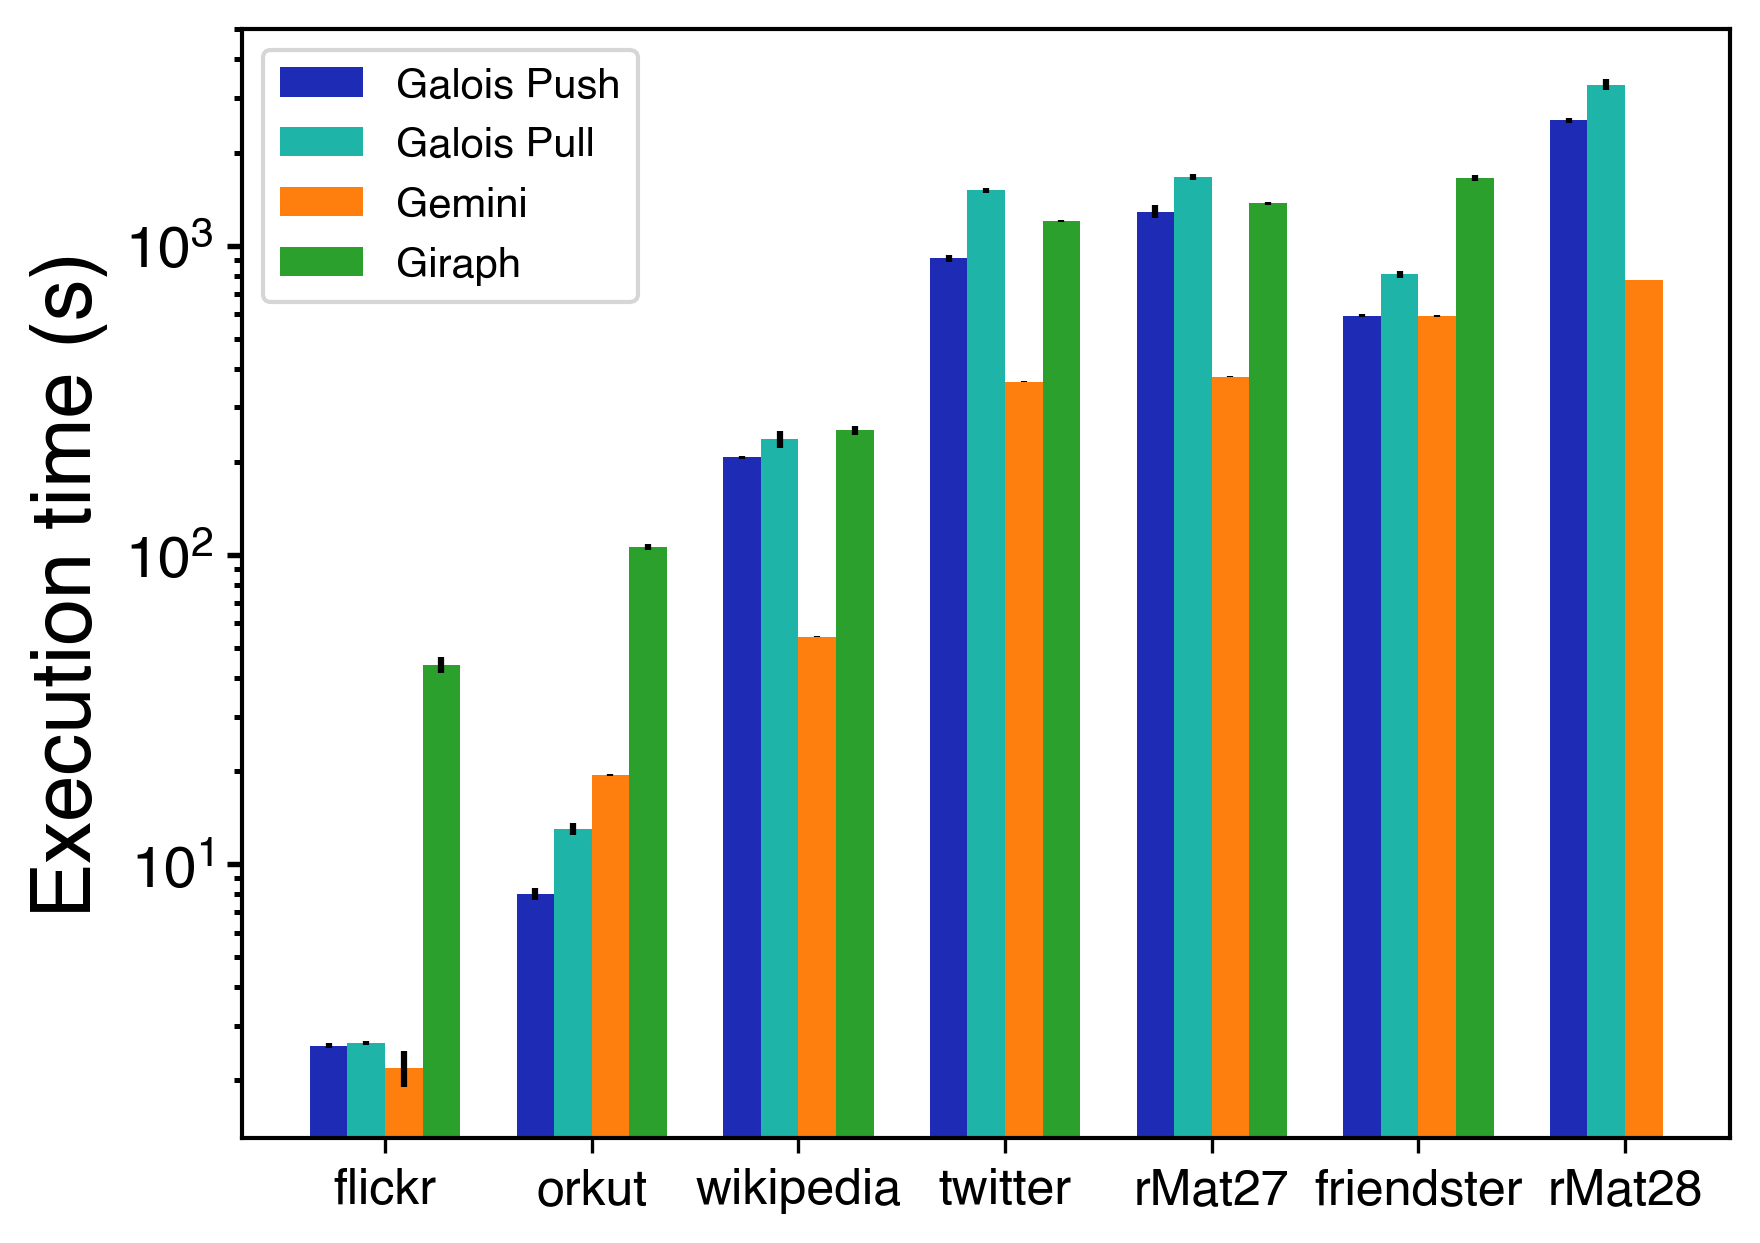
\includegraphics[width=\linewidth]{../../plots/distributedPR_execTime.png}
		\caption{Execution times for distributed PR}
		\label{fig:distributedPR_exec}
	\end{subfigure}
	\hfil
	\begin{subfigure}{0.3\textwidth}
		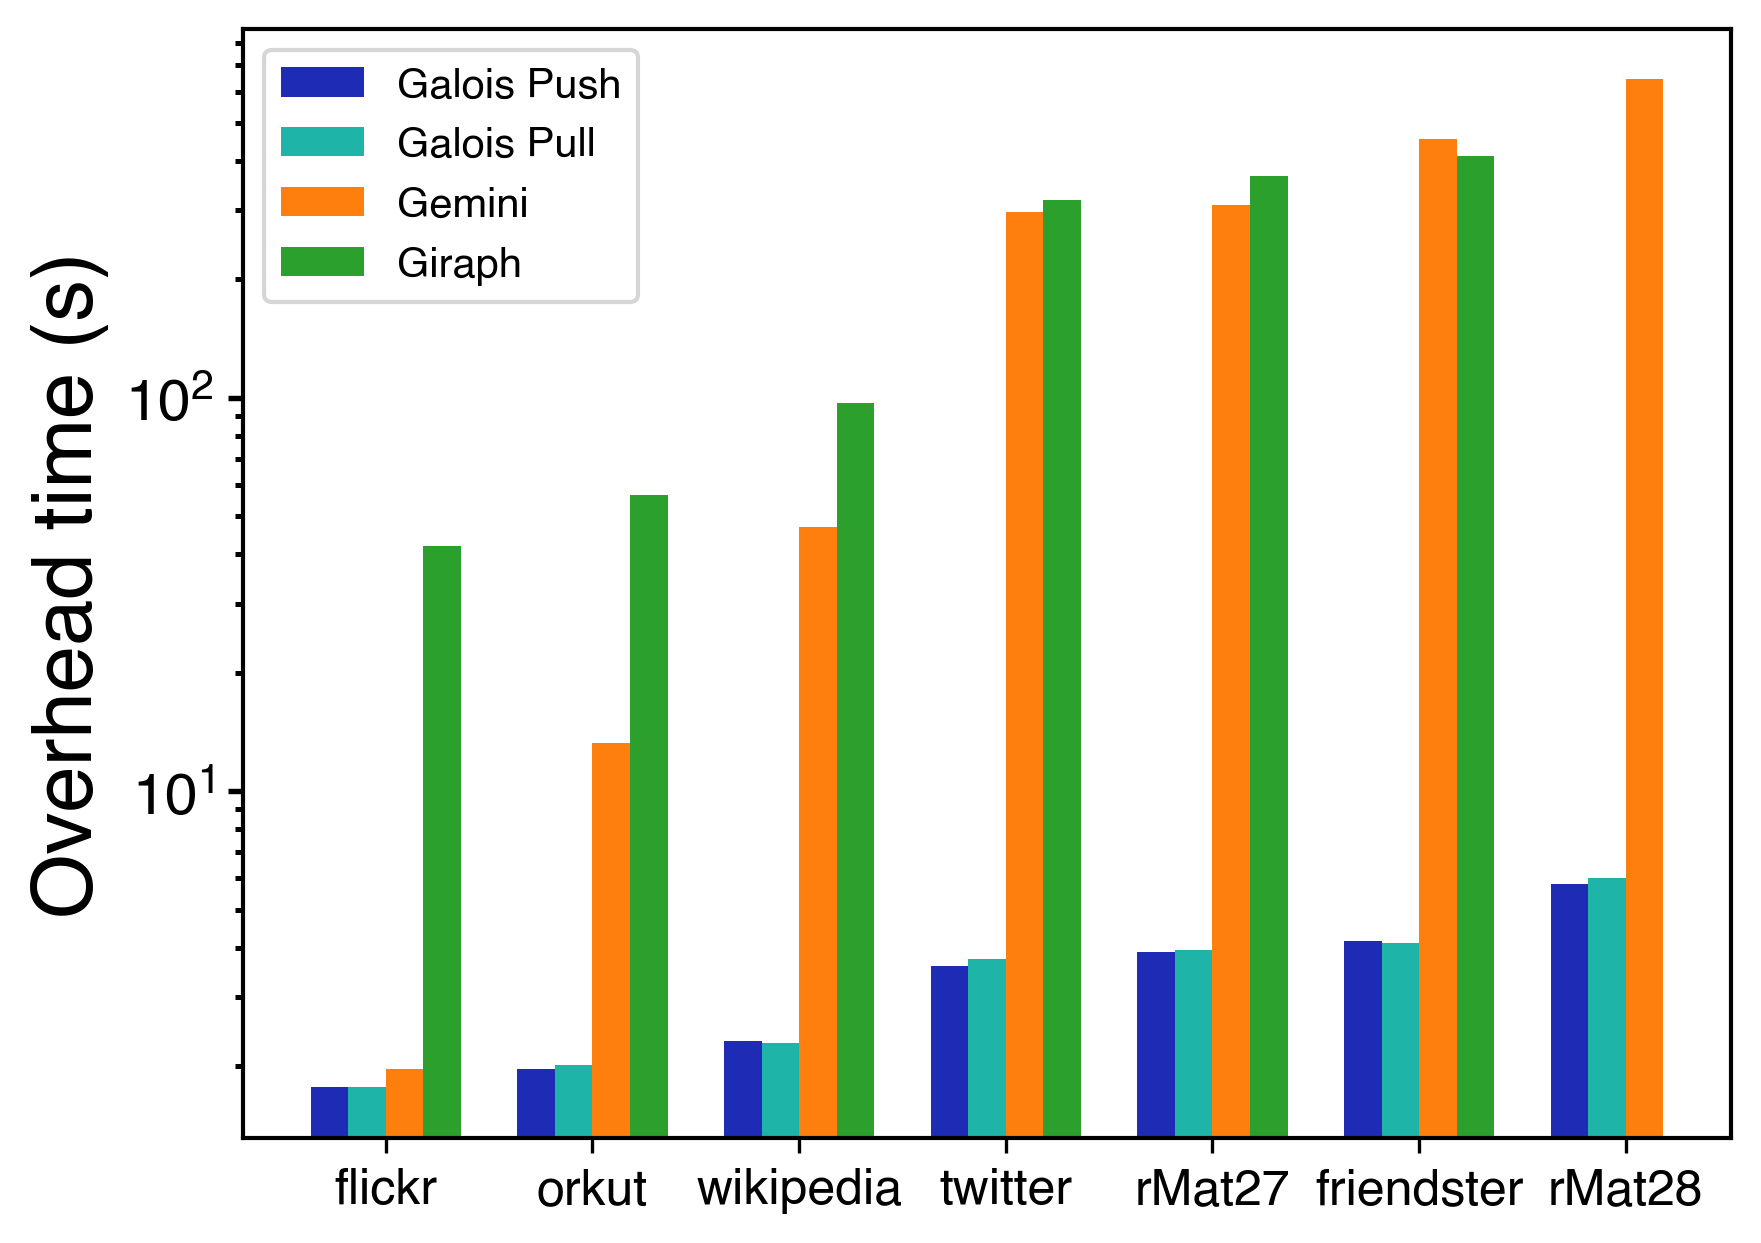
\includegraphics[width=\linewidth]{../../plots/distributedPR_overheadTime.png}
		\caption{Overhead time}
		\label{fig:distributedPR_overheadNormalized}
	\end{subfigure}

	\caption{Average times on the distributed cluster, black bars represent one standard deviation in our testing}
	\label{fig:distributedPR}
\end{figure*}









